\section{Requirements}
\label{sec:requirements}
Als Anforderung wird eine Bedingung oder Eigenschaft bezeichnet, die ein System benötigt, um ein Problem zu lösen oder um einem Standard zu genügen (vgl. IEEE Std 610.12-1990). Drei Arten von Anforderungen sind funktionale Anforderungen, Qualitätsanforderungen und Rahmenbedingungen (vgl. \cite{young}). In diesem Kapitel werde ich zunächst auf bestehende und neu entstandene Anwendungsfälle eingehen und die zugrundeliegenden Anforderungen aufzeigen. Danach möchte ich im Abschnitt \ref{sec:req} einige Qualitätsanforderungen erläutern.

\subsection{Problem Description}
\label{sec:problem}

In order to conceive a flexible, effective and efficient solution, we survey in this section the challenges associated with Wiki syntax, \wik and large-scale extraction.

\subsection{Processing Wiki Syntax}
Pages in \wik are formatted using the \textit{wikitext} markup language\footnote{\url{http://www.mediawiki.org/wiki/Markup_spec}}.
Operating on the parsed HTML pages, rendered by the \emph{MediaWiki engine}, does not provide any significant benefit, because the rendered HTML does not add any valuable information for extraction. 
Processing the database backup XML dumps\footnote{\url{http://dumps.wikimedia.org/backup-index.html}} instead, is convenient as we could reuse the DBpedia extraction framework\footnote{\url{http://wiki.dbpedia.org/Documentation}} in our implementation. The framework mainly provides input and output handling and also has built-in multi-threading by design.
Actual features of the wikitext syntax are not notably relevant for the extraction approach, but we will give a brief introduction to the reader, to get familiar with the topic. 
A wiki page is formatted using the lightweight (easy to learn, quick to write) markup language \textit{wikitext}. 
Upon request of a page, the MediaWiki engine renders this to an HTML page and sends it to the user's browser. 
An excerpt of the \wik page \textit{house} and the resulting rendered page are shown in Figure \ref{fig:wikitext}.

\begin{figure}[tb]
\centering
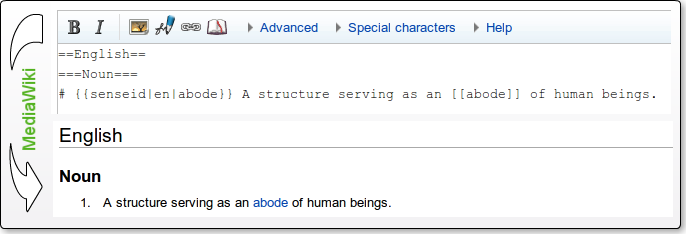
\includegraphics[width=0.9\textwidth]{./images/wikitext.png}
\caption{An excerpt of the \wik page \textit{house} with the rendered HTML.}
\label{fig:wikitext}
\end{figure}

The markup \texttt{==} is used to denote headings, \texttt{\#} denotes a numbered list (\texttt{*} for bullets), \texttt{[[link label]]} denotes links and \texttt{\{\{\}\}} calls a template.
Templates are user-defined rendering functions that provide shortcuts aiming to simplify manual editing and ensuring consistency among similarly structured content elements. 
In MediaWiki, they are defined on special pages in the \texttt{Template:} namespace. 
Templates can contain any wikitext expansion, HTML rendering instructions and placeholders for arguments. 
In the example page in Figure~\ref{fig:wikitext}, the \texttt{senseid} template\footnote{\url{http://en.wiktionary.org/wiki/Template:senseid}} is used, which does nothing being visible on the rendered page, but adds an id attribute to the HTML \texttt{li}-tag (which is created by using \texttt{\#}).
If the English \wik community decides to change the layout of senseid definitions at some point in the future , only a single change to the template definition is required. 
Templates are used heavily throughout \wik, because they substantially increase maintainability and consistency. 
But they also pose a problem to extraction: on the unparsed page only the template name and its arguments are available.
Mostly this is sufficient, but if the template adds static information or conducts complex operations on the arguments (which is fortunately rare), the template result can only be obtained by a running MediaWiki installation hosting the pages. 
The resolution of template calls at extraction time slows the process down notably and adds additional uncertainty.

\subsection{Wiktionary}\label{sec:wiktionary}
\wik has some unique and valuable properties:
\begin{compactitem}
  \item \textbf{Crowd-sourced} \\
    \wik is community edited, instead of expert-built or automatically generated from text corpora. 
    Depending on the activeness of its community, it is up-to-date to recent changes in the language, changing perspectives or new research. 
    The editors are mostly semi-professionals (or guided by one) and enforce a strict editing policy. 
    Vandalism is reverted quickly and bots support editors by fixing simple mistakes and adding automatically generated content. 
    The community is smaller than Wikipedia's but still quite vital (between 50 and 80 very active editors with more than 100 edits per month for the English \wik in 2012\footnote{\url{http://stats.wikimedia.org/wiktionary/EN/TablesWikipediaEN.htm}}). 
   \item \textbf{Multilingual}\\
    The data is split into different Wiktionary Language Editions (WLE, one for each language). 
    This enables the independent administration by communities and leaves the possibility to have different perspectives, focus and localization.
    Simultaneously one WLE describes multiple languages; only the representation language is restricted. 
    For example, the German \wik contains German description of German words \textbf{as well as} German descriptions for English, Spanish or Chinese words. 
    Particularly the linking across languages shapes the unique value of \wik as a rich multi-lingual linguistic resource. 
    Especially the WLE for not widely spread languages are valuable, as corpora might be rare and experts are hard to find.
  \item \textbf{Feature rich}\\
    As stated before, \wik contains for each lexical word (A lexical word is just a string of characters and has no disambiguated meaning yet) a disambiguation regarding language, part of speech, etymology and senses. 
    Numerous additional linguistic properties exist normally for each part of speech. 
    Such properties include word forms, taxonomies (hyponyms, hyperonyms, synonyms, antonyms) and translations.
    Well maintained pages (e.g. frequent words) often have more sophisticated properties such as derived terms, related terms and anagrams.
  \item \textbf{Open license}\\
    All the content is dual-licensed under both the \textit{Creative Commons CC-BY-SA 3.0 Unported License}\footnote{\url{http://en.wiktionary.org/wiki/Wiktionary:Text_of_Creative_Commons_Attribution-ShareAlike_3.0_Unported_License}} as well as the \textit{GNU Free Documentation License (GFDL)}.\footnote{\url{http://en.wiktionary.org/wiki/Wiktionary:GNU_Free_Documentation_License}}
    All the data extracted by our approach falls under the same licences. 
  \item \textbf{Big and growing}\\
    English contains 2,9M pages, French 2,1M, Chinese 1,2M, German 0,2 M.
    The overall size (12M pages) of \wik is in the same order of magnitude as Wikipedia's size (20M pages)\footnote{\url{http://meta.wikimedia.org/wiki/Template:Wikimedia_Growth}}. 
    The number of edits per month in the English \wik varies between 100k and 1M --- with an average of 200k for 2012 so far. 
    The number of pages grows --- in the English \wik with approx. 1k per day in 2012.\footnote{\url{http://stats.wikimedia.org/wiktionary/EN/TablesWikipediaEN.htm}}
\end{compactitem}

The most important resource to understand how \wik is organized are the \textit{Entry Layout Explained} (ELE) help pages.
As described above, a page is divided into sections that separate languages, part of speech etc. 
The table of content on the top of each page also gives an overview of the hierarchical structure. 
This hierarchy is already very valuable as it can be used to disambiguate a lexical word. 
The schema for this tree is restricted by the ELE guidelines\footnote{For English see \url{http://en.wiktionary.org/wiki/Wiktionary:ELE}}. 
The entities illustrated in Figure~\ref{fig:example} of the ER diagram will be called \textit{block} from now on. 
The schema can differ between WLEs and normally evolves over time.

\begin{figure}[tb]
\centering
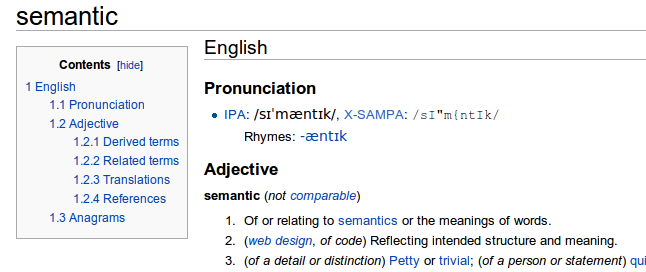
\includegraphics[width=0.9\textwidth]{./images/example-page.png}
\vspace{0.3cm}
\hspace{0.1cm}

\includegraphics[width=0.9\textwidth]{./images/entrylayout.png}
\caption{Example page \texttt{http://en.wiktionary.org/wiki/semantic} and underlying schema (only valid for the English \wik, other WLE might look very different.)}
\label{fig:example}
\end{figure}

\subsection{Wiki-scale Data Extraction}
The above listed properties that make \wik so valuable, unfortunately pose a serious challenge to extraction and data integration efforts. 
Conducting an extraction for specific languages at a fixed point in time is indeed easy, but it eliminates some of the main features of the source. 
To fully synchronize a knowledge base with a community-driven source, one needs to make distinct design choices to fully capture all desired benefits.
MediaWiki was designed to appeal to non-technical editors and abstains from intensive error checking as well as formally following a grammar --- the community gives itself just layout guidelines. 
One will encounter fuzzy modelling and unexpected information. 
Editors often see no problem with such "noise" as long as the page's visual rendering is acceptable.  
Overall, the main challenges can be summed up as (1) the constant and frequent changes to data \textit{and schema}, (2) the heterogeneity in WLE schemas and (3) the human-centric nature of a wiki. 

\newpage
